%!TEX program = lualatex
\documentclass[12pt, a4paper, oneside]{report}
\usepackage{amsmath}
\usepackage{fontspec}
\usepackage[top=2cm, bottom=2cm, left=2cm, right=2cm]{geometry}

\setmainfont{Times New Roman}
\usepackage{graphicx}
\usepackage{subcaption}
\usepackage[style=apa, backend=biber]{biblatex}

\usepackage{titlesec}
\usepackage{booktabs}
\usepackage{float}
\usepackage{listings}
\usepackage{enumitem}
\usepackage{multirow}
\usepackage{tabularx} 

\lstset{
  breaklines=true,
  basicstyle=\ttfamily\small,
  columns=fullflexible
}

\titleformat{\chapter}[display]
  {\normalfont\huge\bfseries}{}{0pt}{\Huge}
\titlespacing*{\chapter}{0pt}{-50pt}{20pt}


\begin{document}


\begin{titlepage}
    \begin{center}
        \vspace*{1cm}
        
        % --- Title ---
        \Huge
        \textbf{PART 1: Thesis} \\
        \vspace{1cm}

    \end{center}
\end{titlepage}

\begin{titlepage}
    \begin{center}
        \vspace*{1cm}
        
        % --- Title ---
        \Huge
        \textbf{PART 2: Internship Report} \\
        \vspace{1cm}
        
        % --- Subtitle/Role ---
        \Large
        Role: Data Science Intern \\
        \vspace{2cm}
        
        % --- Company & Supervisor ---
        \huge
        \textbf{Company: Vodafone} \\
        \vspace{0.5cm}
        \textbf{Supervisor: Spiros Aravanis}

    \end{center}
\end{titlepage}


% --- Table of Contents ---
\tableofcontents
\newpage



\chapter{Introduction}
	
\subsection{Company Description}
Vodafone is one of the world's leading telecommunications companies, providing communication and digital services across Europe and Africa. The company has evolved from a traditional mobile network operator into a technology company that offers a broad portfolio of connectivity and digital solutions. Its strategy focuses on providing reliable communication services, investing in network infrastructure, and supporting the digital transformation of both individuals and businesses.

The company's operations are based on extensive mobile and fixed network infrastructure, which enables millions of customers to communicate, access the internet, and use digital services every day. Continuous investments in fiber networks, 5G technology, cloud platforms, and cybersecurity allow Vodafone to improve network performance while responding to the increasing demand for faster and more secure connectivity. Besides telecommunications services, Vodafone also develops digital platforms and solutions that help customers simplify everyday activities and improve productivity.

Vodafone Greece is the Greek subsidiary of the Vodafone Group and has been operating in the Greek telecommunications market for more than three decades. The company provides nationwide mobile and fixed telecommunications services, broadband internet, fiber connections, television services, and digital applications. Through continuous investments in its network infrastructure and customer services, Vodafone Greece aims to strengthen its position in a highly competitive market while supporting the country's digital transformation. The company serves millions of subscribers and continuously expands its fiber and 5G coverage to improve connectivity across Greece.

\subsection{Core Activities and Customer Segments}
Vodafone's main business activity is providing communication services through mobile and fixed telecommunications networks. However, the company has expanded beyond traditional telecommunications by offering cloud computing, cybersecurity, Internet of Things (IoT), unified communications, and managed digital services. These activities allow Vodafone to operate not only as a network provider but also as a technology partner for individuals, businesses, and public organizations.

Vodafone serves two main customer segments: Business-to-Consumer (B2C) and Business-to-Business (B2B). The B2C segment focuses on individual customers and households by offering mobile subscriptions, prepaid plans, broadband internet, fiber connections, television services, and digital applications. These services are designed to provide reliable connectivity for communication, entertainment, remote work, and everyday digital activities.

The B2B segment focuses on companies of all sizes, from small businesses to large enterprises and public organizations. Business customers require more than basic connectivity, as they depend on secure and reliable communication systems to support their daily operations. Vodafone offers solutions such as corporate mobile and fixed communications, cloud infrastructure, cybersecurity services, IoT applications, private networks, and collaboration platforms. For example, a logistics company may use IoT solutions to monitor its vehicle fleet, while a retail company can connect multiple stores through secure private networks. Healthcare providers, banks, and manufacturing companies also use Vodafone's digital services to improve efficiency, security, and communication.

By serving both consumer and business markets, Vodafone has developed a diversified business model that combines telecommunications with digital technologies. This approach enables the company to respond to changing customer needs while maintaining its role as one of the leading providers of connectivity and digital services.

\subsection{ Strategic Initiatives in Greece}
Currently, Vodafone Greece complements its telecommunications services through several strategic initiatives. The company continues to invest in submarine fiber optic infrastructure, including the connection of Crete with mainland Greece through the Thetis cable system, strengthening the country's digital connectivity and increasing network resilience. Vodafone also promotes safer internet use through its partnership with Qustodio, which provides parents with tools to monitor and manage their children's online activity according to their age and development. In addition, the Vodafone Posidonia program uses advanced technology and the Vodafone 5G network to map and monitor Posidonia oceanica seagrass meadows, contributing to marine research and the protection of one of the Mediterranean's most valuable ecosystems. These initiatives demonstrate that Vodafone's role extends beyond providing communication services by supporting digital innovation, social responsibility, and environmental sustainability.

\subsection{Internship Objective}
The main objective of the internship was to gain a practical understanding of how data science is applied in a large multinational company. Throughout university studies, data science emerged as one of the most interesting fields due to its combination of programming, statistics, and business decision making. The internship provided the opportunity to observe how analytical methods are used to solve real business problems, support decision making, and create value for both the company and its customers.

Vodafone was selected because it operates on a global scale while making extensive use of data across many business functions, including customer analytics, network optimization, and commercial strategy. This offered the opportunity to experience how technical solutions are developed within a structured corporate environment and how different departments collaborate to achieve common business objectives.

Beyond the technical aspect, another important goal was to understand the professional environment of a large organization. This included learning how projects are planned, how work is organized to meet deadlines, how progress is communicated within a team, and how collaboration takes place between employees with different areas of expertise. Particular emphasis was placed on developing the ability to communicate technical concepts and analytical results to colleagues without a technical background, ensuring that data-driven insights could support business decisions effectively.

Overall, the internship aimed to strengthen both technical and professional skills while providing a broader understanding of how data science, business objectives, and teamwork are integrated within a modern technology company.

% PARAGRAPH EXPLAINING THE PURPOSE OF THIS REPORT

\section{Department}
\subsection{Commercial Business Unit}
The internship was carried out within the Commercial Business Unit (CBU), a key division responsible for managing Vodafone’s customer base and supporting commercial decision-making across products and services. The unit plays a central role in ensuring that customer needs are aligned with business objectives while also maintaining sustainable growth across both mobile and fixed-line services.

From a structural perspective, the CBU is organized around the full customer lifecycle, starting from acquisition and extending to customer engagement and retention. Mobile services are generally divided into prepaid and contract (postpaid) customers, while fixed services include broadband internet, converged offers, and television subscriptions.


A strong focus of the unit is data-driven decision making. Within this environment, multiple teams work together to support marketing and commercial operations. The Customer Value Management (CVM) function is responsible for monitoring overall customer performance, identifying behavioural trends, and ensuring that commercial actions are aligned with financial and strategic targets. This includes analysing key indicators such as customer retention, product usage, and market response to different campaigns.

A significant part of the analytical work is supported by the Big Data team, where the internship was conducted. This team focuses on developing analytical models that help predict customer behaviour. Typical applications include estimating the likelihood of customer churn, identifying potential response rates to marketing campaigns, and segmenting customers based on behavioural patterns. These outputs are essential for defining the target groups used in commercial actions.

Once analytical models generate target audiences, the campaign lists are further refined through additional validation processes. This step ensures that business rules, communication policies, and operational constraints are respected before any customer interaction takes place. This coordination ensures that campaigns are not only data-driven but also aligned with strategic and regulatory requirements.


\subsection{Role}
The role of Data Scientist within the Big Data team focused on supporting analytical workflows used for segmentation and visualization. The introduction into the company included mandatory HR training course according to behavioral standards such as inclusivity, and security attack lessons like phishing and social engineering. After completing this step, virtual lessons relevant to what my team used regarding Machine Learning algorithms and tools were high suggested to make sure everyone was in the right page according to the team’s best practices. In order to finalize the internship’s project, each team member made sure to inform me about their running projects and current achievements. 

Since in Vodafone each employee focuses in one product (pre-paid, post-pay, fixed) and after a meeting with my supervisor and the Big Data Manager, it was most fit for my interests to be assigned a project in the fixed segment. More specifically, I was responsible of creating an existing project in the mobile segment, which was the geographical segmentation of Greece based on the customers fixed network experience, as well as identifying possible relationships with the populations’ demographics.

The position required a combination of technical and professional skills. On the technical side, familiarity with data analysis concepts, programming for data processing, and basic understanding of machine learning principles were important. As a data scientist, it was also critical to be able to understand and configure business thresholds and other metrics in order to create value. On the professional side, strong communication skills, structured thinking, and the ability to work within deadlines were essential. In addition, attention to detail and the ability to translate analytical results into business insights were key components of the role.

The main expected outcome of the internship work was to contribute to the development and refinement of data-driven customer insights used in commercial decision-making. More broadly, the role aimed to support the improvement of targeting network weaknesses on prefecture and zip-code level based on quality metrics and customer experience. The final deliverable was a map visualization of Greece, cloring each geographical component in different colors, in order to get a quick overview of Vodafone’s fixed network experience. A second eye would be able to see which areas are problematic and why, making the improvement plants more targeted and efficient. 


\chapter{Projects}

\section{Activities}
The internship was carried out within the fixed segment of the Commercial Business Unit, where one main analytical project was undertaken: the Geographical Segmentation and Customer Experience Analysis. The aim of the project was to segment the customer base at prefecture and ZIP-code level in order to identify how network experience varies across the country and how it relates to demographic characteristics. It would also result in identifying the best and worst quality areas, which could open a conversation about future strategy. Alongside the core analysis, the corporate setup required two recurring activities: weekly updates on the project's progress to the team, and a final presentation of the methodology and findings to the whole team. An initial familiarization period was also needed in order to understand the company's data structures, naming conventions and the way each field is defined internally.

The sections that follows concentrate on the two most substantial activities: the analytical project itself and the reporting and presentation work that accompanied it.

\section{Results}

\subsection{Geographical Segmentation and Customer Experience Analysis}
The project was based on two datasets. The first one described customers and contained geographic, product, usage, quality, pricing and experience information across roughly 700,000 records. The second one listed demographic information at ZIP-code level, such as population, purchasing power and household size. The first task was therefore to merge the two sources into a single dataset based on ZIP code.

\subsubsection{Pre-processing} 
Because a large share of records carried missing or inconsistent location values, prefecture was adopted as the reference point for correctness: where the most common prefecture of a ZIP did not match the recorded one, the ZIP and city were treated as wrong and reset. For records with no valid ZIP, a spatial join (sjoin) matched customer coordinates to ZIP-code polygons. The rest of the cleaning handled nulls, negative values and logically inconsistent entries, for example cases where the initial tenure was lower than the renewal tenure, always taking into account how each field is defined by the company. Unique values and ranges were explored to understand the meaning of each variable, and outliers were replaced with medians or zeros depending on the field. Speed outliers were treated separately, using thresholds per technology and nominal speed so that legitimate high-speed values were not removed.

\subsubsection {Exploratory data analysis.}
Identifying correlations and dependencies between variables was essential in order to avoid introducing bias or distortion into the analysis. Given the range of products in the fixed segment, every exploration was split by product type (ADSL, FTTC, FTTH) and connection speed (24, 50, 100~Mbps and above). Group-by summaries and cumulative distribution plots were the main tools used to understand customer behaviour within each category and to identify natural breakpoints in the data.

\subsubsection{Feature engineering} 
The next step was to decide which fields could meaningfully describe customer experience. After examining their distribution and impact, the analysis was built around four key indicators: speed, disconnections, attenuation and complaints. Each customer metric was binned into high, medium and low levels using business-driven thresholds, and competitor products were combined with Vodafone's so that technologies could be compared on a like-for-like basis. These customer-level bins were then aggregated to ZIP and prefecture level as the share of high, medium and low customers per metric, together with weighted averages and product-mix percentages. A vital step for this analysis is to do the above binning different per product type and speed, so that the results are not because a customer or area has a cheaper/ weaker product but because this product is of lower quality based on business standards. If this step was not considered, it would be obvious that FTTH areas would have better quality and ADSL worse not according to the network quality but due to technology (ftth has no attenuation and speed range above 100 while ADSL has a maximum speed of 24).

\subsubsection {Segmentation} 
A score was produced for each metric from its bin distribution ($\text{Score} = 2\cdot\text{High\%} + 1\cdot\text{Medium\%} + 0\cdot\text{Low\%}$), and the metric scores were combined into a single total score using weights derived from Principal Component Analysis (PCA), so that the indicators explaining most of the variation between areas carried the most weight. 
\begin{equation}
\mathrm{PC1}=w_1\mathrm{SpeedScore}+w_2(2-\mathrm{AttenuationScore})+w_3(2-\mathrm{DisconnectionsScore})+w_4(2-\mathrm{ComplaintsScore})
\end{equation}
Areas were then ranked by total score and split into High, Medium and Low quality segments at both ZIP-code (860 areas) and prefecture (51 areas) level. The segments were finally profiled against the demographic data, which showed that higher-quality networks are concentrated in smaller-household, higher-purchasing-power areas.

\subsubsection{Best practices and key methods / tools}
The work was carried out in Python woking inside an jupyter notebook environment, mainly with pandas for data manipulation, geopandas for the spatial join between coordinates and ZIP polygons, and scikit-learn for the PCA used to set the scoring weights. Matplotlib was used for the cumulative plots and Kepler for segment visualisations. On the methodological side, the main practices were: treating one trusted field (prefecture) as a baseline to repair the rest, cleaning each variable according to its business definition rather than applying blanket rules, analysing metrics by technology and nominal speed to keep comparisons fair, and using a transparent, rule-based scoring scheme whose weights were justified statistically through PCA rather than chosen by hand.

Once the segments were defined, each segmented data frame was described through the metrics it carried. For every segment the frame held the per-metric scores and the weighted averages of the underlying KPIs (speed, usage, disconnections, attenuation, complaints and bill), together with the operator and technology mix and the average number of customers per area. The pattern across segments was consistent: as quality fell, the average speed dropped (from roughly 78 to 55~Mbps between high- and low-quality ZIP codes) while disconnections and attenuation rose, whereas complaints and bills stayed comparatively flat. This confirmed that speed, disconnections and attenuation were the metrics that separated the segments most clearly.
 
\subsubsection{Demographic profiling} 
The segments were finally profiled against the demographic fields merged from the ZIP-level dataset. Higher-quality areas were associated with higher purchasing power and smaller households, while lower-quality areas showed the opposite, pointing to congestion in larger, more densely populated households where usage and disconnections were higher and speed lower. At prefecture level these differences smoothed out, as the aggregation averaged away the contrasts that were visible between individual ZIP codes.


\subsubsection{Deliverables}
The activity produced a single cleaned and merged dataset at customer level, and two segmented data frames, one at ZIP-code level and one at prefecture level, each containing the segment label, the total and per-metric scores, the weighted KPI averages, the demographic averages and the product-mix percentages. These were accompanied by the documented scoring and segmentation methodology and by the ranked lists of best- and worst-quality areas that fed the final presentation.


\section{Impact on the Business Operation}
The activity converted around 700,000 raw customer records and the accompanying demographic data into an area-level view of network quality, covering 860 ZIP codes and 51 prefectures. By ranking these areas and isolating the metrics that drive quality the most (speed, disconnections and attenuation), the analysis gives the business a single, evidence-based reference for where the fixed network performs well and where it underperforms. This supports more targeted decisions on infrastructure investment and resource allocation, since effort can be directed to the areas and indicators that matter most rather than spread evenly across the country.

\subsection{Weekly Reporting and Final Presentation}
\subsubsection{Activity description}
Throughout the project, progress was reported to the team on a weekly basis. Each update summarized the stage reached, the decisions taken and any open questions or bugs, which kept the analysis aligned with business expectations and allowed methodological choices to be validated early. At the end of the internship, the full methodology and findings were presented to the whole team in a single session.

\subsubsection{Best practices and key methods / tools}
The reporting relied on clear, concise summaries of each stage rather than raw output. The final deck was built around a simple narrative, moving from the data sources and cleaning, through feature engineering and scoring, to the segments and the demographic insights, using consistent visuals (cumulative plots, segment pie charts and operator-mix bars) so that a non-technical audience could follow the reasoning. PowerPoint was used for the deck.

\subsubsection{Deliverables}
The deliverables were the recurring weekly progress updates and a final presentation deck covering the use case, the data landscape, the pre-processing, the feature engineering, the ZIP and prefecture segmentation, and the key insights.

\begin{table}[h]
\centering
\begin{tabular}{lccc}
\hline
\textbf{Task Name} & \textbf{Duration} & \textbf{Start} & \textbf{Finish} \\
\hline
Dataset Formulation (Merge \& Spatial Join) & 2 weeks & 11/03/2025 & 22/03/2025 \\
Data Cleaning \& Pre-processing & 2 weeks & 25/03/2025 & 06/04/2025 \\
Exploratory Data Analysis & 1 week & 07/04/2025 & 14/04/2025 \\
Feature Engineering & 2 weeks & 15/04/2025 & 30/04/2025 \\
ZIP \& Prefecture Segmentation & 2 weeks & 04/05/2025 & 19/05/2025 \\
Segment \& Demographic Analysis & 1 week & 20/05/2025 & 25/05/2025 \\
Visualization \& Final Presentation Preparation & 1 week & 25/05/2025 & 28/05/2025 \\
Weekly Progress Reporting & 11 weeks & 10/03/2025 & 28/05/2025 \\
\hline
\end{tabular}
\caption{Tasks during the ZIP \& Prefecture Segmentation}
\label{tab:tasks}
\end{table}

\begin{figure}[H]
\centering
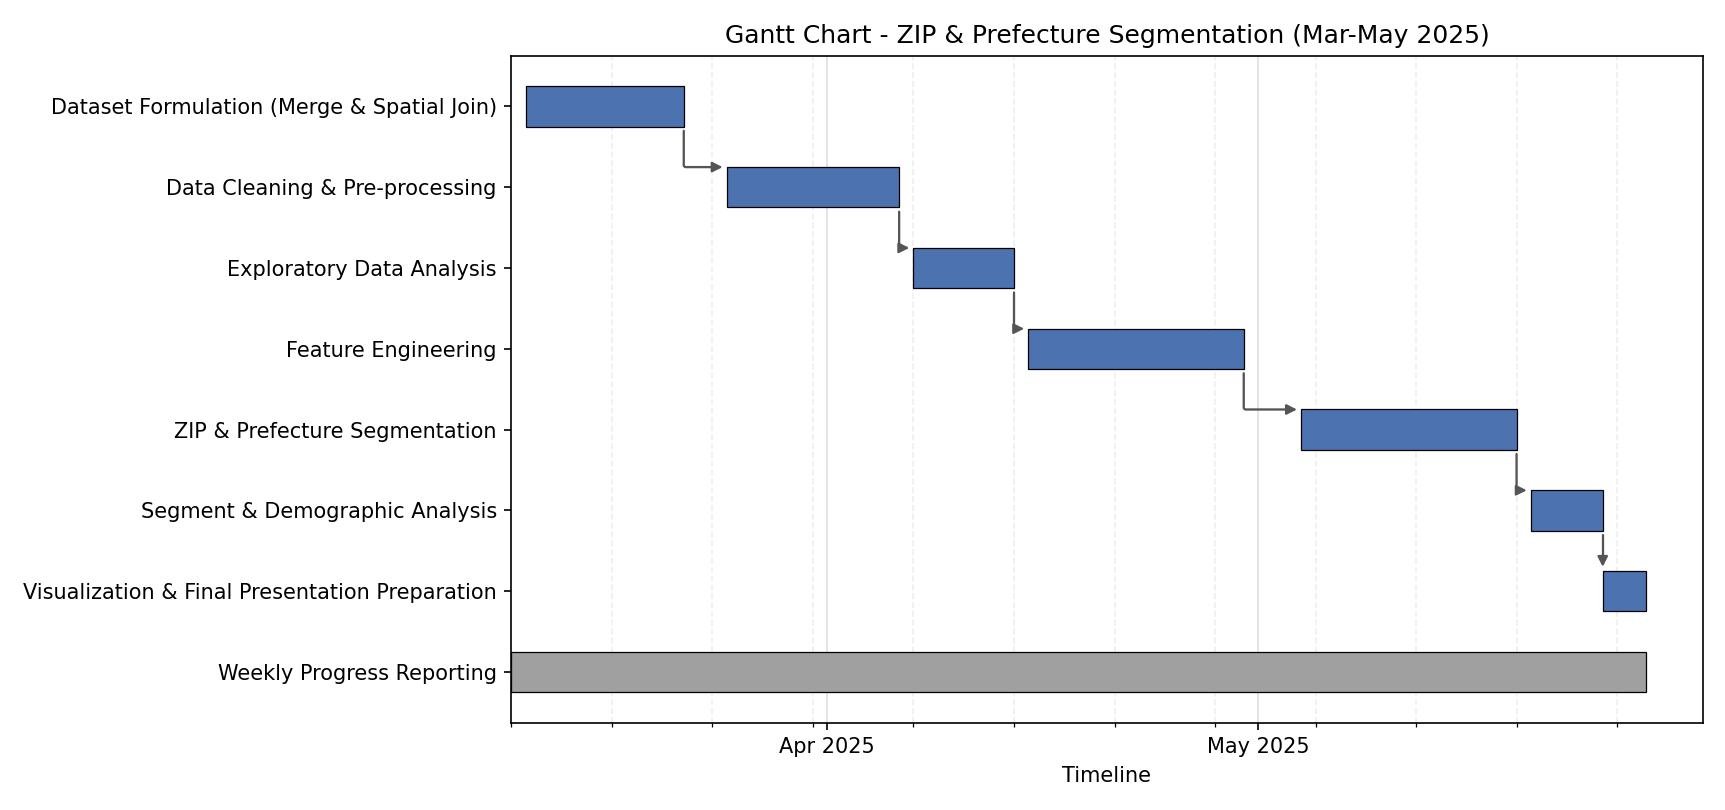
\includegraphics[width=0.8\textwidth]{./gantt_chart.png}
\caption{Truncation rate versus false-positive rate across Generator budgets.}
\end{figure}


\section{Skills Developed}
The internship combined technical and business-oriented work, which allowed a broad set of skills to be developed and applied in practice. Each of the skills listed below was exercised directly within the geographical segmentation project, from preparing and modelling the data through to interpreting the results and communicating them to the team. The table summarises these skills, the main methods associated with each and a concrete example of how they were applied.

\chapter{Skills}
CHECK TABLE CONTENT

\begin{table}[h]
\centering
\renewcommand{\arraystretch}{1.4}
\begin{tabularx}{\textwidth}{p{3.1cm} X X}
\hline
\textbf{Skill} & \textbf{Related Methods} & \textbf{Example} \\
\hline
Applied Machine Learning & Feature engineering, Principal Component Analysis (PCA), threshold and percentile binning (scikit-learn) & PCA used to derive the weights that combine the KPI scores into a single network-quality score. \\
Business Analytics \& Personalization Technologies & Customer segmentation, KPI scoring, exploratory data analysis, group-by aggregation & Classifying 860 ZIP codes and 51 prefectures into High, Medium and Low quality segments for targeted action. \\
Quantitative Methods in Economics and Business & Descriptive statistics, correlation analysis, weighted averages, distribution and percentile analysis & Correlating network KPIs with demographic factors such as purchasing power and household size. \\
Management Science & Rule-based and multi-criteria scoring, prioritisation, resource-allocation analysis, project scheduling & A transparent scoring model that ranks areas to guide infrastructure investment and resource allocation. \\
Business Strategy & Gap analysis, value proposition, competitive and market positioning & Identifying under-served, high-value areas where network quality lags demand, to inform investment priorities. \\
Presentation Skills & Data storytelling, data visualisation, stakeholder communication & Weekly progress updates and a final presentation translating technical findings into clear visuals for a non-technical audience. \\
\hline
\end{tabularx}
\caption{Skills developed during the internship}
\label{tab:skills}
\end{table}


\chapter{Comments and Observations}
\subsection{Work Environment}
The internship took place at Vodafone Greece's headquarters in Chalandri, within the Big Data team of the Commercial Business Unit (CBU). The department operates in a modern corporate environment where business decisions are strongly supported by data analysis and collaboration between technical and commercial teams. The internship followed a hybrid working model, with approximately 40\% of the working hours spent in the office and the remaining time working remotely. This arrangement offered the flexibility of remote work while maintaining regular in-person interaction, which helped strengthen communication, collaboration, and team integration. Throughout the internship, particular emphasis was placed on data confidentiality and information governance, as all analyses were performed using anonymised customer data and in accordance with the company's security policies.

Communication within the department was structured through regular meetings at different organisational levels. Weekly Commercial Business Unit meetings provided updates on business performance, market developments, and competitor activity, allowing employees to better understand the company's commercial strategy. Beyond the department itself, there were opportunities to collaborate with other teams, including Human Resources, through activities organized for Vodafone's internship program. These interactions provided a broader understanding of the company's culture and the cooperation between different business functions.

The office follows an open-plan layout where workstations are informally organized into team areas rather than assigned desks. Although employees have flexibility in choosing where to work, members of the same team usually sit together to facilitate communication and collaboration. This arrangement encouraged spontaneous discussions, quick problem solving, and continuous knowledge sharing throughout the internship. Working in close proximity to experienced data scientists and analysts made it easy to ask questions, validate ideas, and receive immediate feedback, contributing to both the efficiency of the project and the overall learning experience.

\subsection{Operation of the Department}
The department operates as an analytics-supported function, where customer, network and commercial data are used to inform decisions on the fixed-line portfolio. The team consisted of 9 people and their responsibilities were assigned based on products.  This setting provided an autonomous workflow and a deeper understanding of each project, since each member was “specialized” in one product type. 

Work followed a clear weekly rhythm: progress was reviewed in regular team updates, which kept tasks aligned with business priorities and allowed methodological choices to be checked early rather than only at the end. A highlight of the team’s weekly agenda was the brainstorming meetings, where we would focus on one or two running projects in detail and learn from   or solve any questions, creating  a deeper understandingof data science and the company’s needs. Separate meetings with the internship supervisor were organized to review progress, receive feedback, and plan the next stages of the project.

\subsection{Facilitating Factors}
Several factors contributed to the successful completion of the internship. First, the project followed a structured feedback process, with weekly meetings that allowed progress to be reviewed regularly and ensured that the analysis remained aligned with the project's objectives. Receiving continuous feedback at each stage reduced the risk of unnecessary work and made it easier to refine the methodology whenever needed.

Another important factor was the support provided by the Big Data team. Team members were always approachable and willing to explain technical concepts, business terminology, and the meaning of internal datasets whenever clarification was required. This collaborative environment made it easier to understand the business context behind the data rather than focusing only on the technical aspects of the analysis.

The guidance of the internship supervisor also played a significant role. Since the supervisor was responsible for the fixed segment, project discussions, technical guidance, and progress updates were coordinated through a single point of contact, making communication efficient and ensuring that business requirements were clearly understood. Although Vodafone promotes an onboarding process where new employees are introduced to the team and supported during their first weeks by the help of an assigned “buddy”, the integration into the department occurred naturally through daily collaboration with all team members. This created a welcoming environment where questions could be addressed openly and knowledge was shared continuously. Vodafone's onboarding process is designed to help new employees integrate into the company and become familiar with its culture and ways of working.

Finally, the academic background developed throughout the university program, particularly in data analysis, machine learning, and statistics, provided a solid foundation for understanding the analytical tasks and adapting quickly to the tools and methodologies used during the internship.

\subsection{Obstacles and Difficulties}
No major difficulties arose in out of the ordinary workflow. As discussed above, the teams weekly agenda, collaboration, work ethic and culture formed a space were communication solved any hurdles.  For instance, a large share of records carried missing or inconsistent location values, and the geographic fields (ZIP, city, prefecture) did not always align, which made the early merging and cleaning stages more demanding and time-consuming than expected. However, when making the problem aware, only quick brainstorming sessions were required for the solution to emerge.

\subsection{Knowledge and Experience Gained}
The internship provided the opportunity to strengthen both technical and professional skills by applying academic knowledge to real business problems. From a technical perspective, valuable experience was gained in preparing and analysing large datasets, performing exploratory data analysis, engineering new features, and working with geospatial data through spatial joins. The project also introduced the complete analytical workflow, from understanding business requirements and processing raw data to developing meaningful geographical segments and presenting the final results through interactive visualisations. In addition, the analysis required the interpretation of telecommunications network KPIs and the definition of business thresholds, demonstrating how technical methods can support commercial decision making.

Beyond the technical aspects, the internship offered a valuable introduction to the dynamics of a large corporate environment. Experience was gained in organizing work around deadlines, reporting progress regularly, and communicating analytical results to colleagues with different professional backgrounds. An important lesson was learning how to explain technical concepts in a clear and understandable way so that they could support business discussions and decision making.

The collaborative culture of the Big Data team also had a significant impact on the overall learning experience. Knowledge sharing was encouraged, allowing new ideas and analytical approaches to be discussed openly among team members. This created an environment where learning was a continuous process and where every member was encouraged not only to acquire new knowledge but also to contribute back to the team. As a result, the internship demonstrated that effective teamwork extends beyond meeting project deadlines and relies on communication, trust, and continuous professional development.

\subsection{Suggestions for Improvement}
Overall, the working environment and team structure were well organized and effective, with no major issues identified during the internship period. However, one potential area for enhancement concerns documentation practices. More detailed and centralized documentation of datasets, ongoing projects, internal processes, and product definitions could further improve onboarding efficiency for new team members or employees joining an existing project. This would allow faster familiarization with both the technical and business context of the work.

Apart from this aspect, the working approach within the team was flexible and supportive, allowing members to explore different analytical methods and contribute creatively to ongoing tasks. This balance between structure and autonomy created a productive environment that supported both individual development and team objectives.

\end{document}
